\documentclass{article}
\usepackage[utf8]{inputenc} %кодировка
\usepackage[T2A]{fontenc}
\usepackage[english,russian]{babel} %русификатор 
\usepackage{mathtools} %библиотека матеши
\usepackage[left=1cm,right=1cm,top=2cm,bottom=2cm,bindingoffset=0cm]{geometry} %изменение отступов на листе
\usepackage{amsmath}
\usepackage{graphicx} %библиотека для графики и картинок
\graphicspath{}
\DeclareGraphicsExtensions{.pdf,.png,.jpg}
\usepackage{subcaption}
\usepackage{pgfplots}

\begin{document}
% НАЧАЛО ТИТУЛЬНОГО ЛИСТА
\begin{center}
    \Large
    Федеральное государственное автономное \\
    образовательное учреждение высшего образования \\ 
    «Научно-образовательная корпорация ИТМО»\\
    \vspace{0.5cm}
    \large
    Факультет программной инженерии и компьютерной техники \\
    Направление подготовки 09.03.04 Программная инженерия \\
    \vspace{1cm}
    \Large
    \textbf{Отчёт по лабораторной работе №1} \\
    По дисциплине "Web программирование" \\
    \large
    \vspace{8cm}

    \begin{minipage}{.33\textwidth}
    \end{minipage}
    \hfill
    \begin{minipage}{.4\textwidth}
    
        \textbf{Студент}: \vspace{.1cm} \\
        \ Дениченко Александр P3212\\
        \textbf{Практик}:  \\
        \ Харитонова А. Е.
    \end{minipage}
    \vfill
Санкт-Петербург\\ 2023 г.
\end{center}

% КОНЕЦ ТИТУЛЬНОГО ЛИСТА 
\newpage

\section{Задание}
% 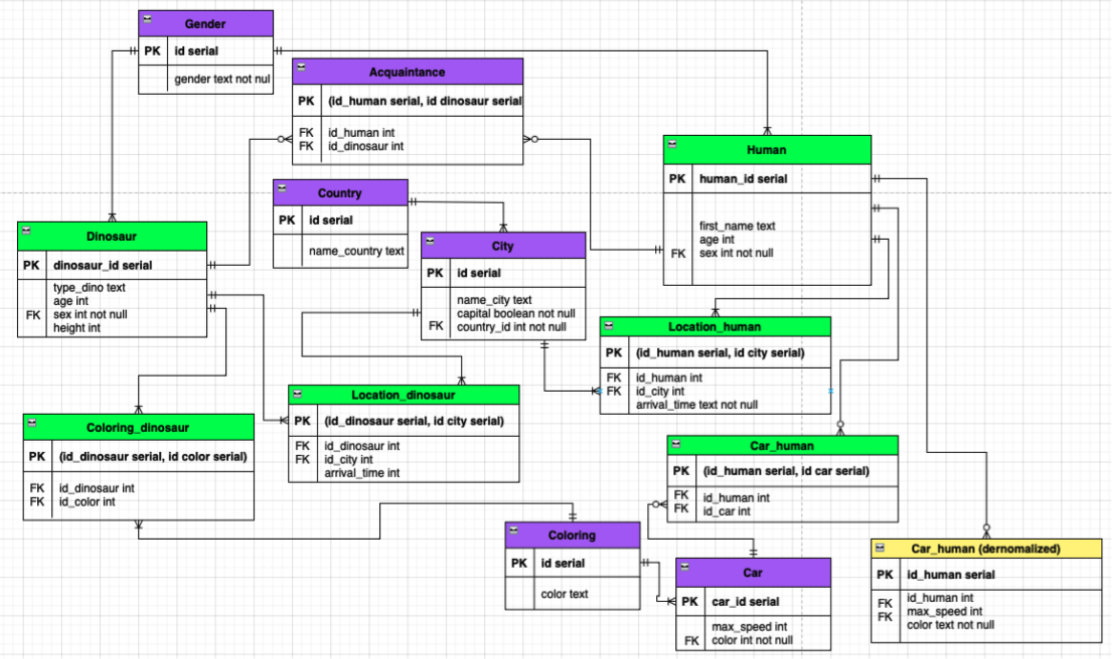
\includegraphics[width=.9\textwidth]{123}
Разработать PHP-скрипт, определяющий попадание точки на координатной плоскости в заданную область, и создать HTML-страницу, которая формирует данные для отправки их на обработку этому скрипту.




Параметр R и координаты точки должны передаваться скрипту посредством HTTP-запроса. Скрипт должен выполнять валидацию данных и возвращать HTML-страницу с таблицей, содержащей полученные параметры и результат вычислений - факт попадания или непопадания точки в область. Предыдущие результаты должны сохраняться между запросами и отображаться в таблице.



Кроме того, ответ должен содержать данные о текущем времени и времени работы скрипта.


Разработанная HTML-страница должна удовлетворять следующим требованиям:


Для расположения текстовых и графических элементов необходимо использовать табличную верстку.


Данные формы должны передаваться на обработку посредством GET-запроса.


Таблицы стилей должны располагаться в самом веб-документе.


При работе с CSS должно быть продемонстрировано использование селекторов псевдоэлементов, селекторов дочерних элементов, селекторов классов, селекторов атрибутов а также такие свойства стилей CSS, как наследование и каскадирование.


HTML-страница должна иметь "шапку", содержащую ФИО студента, номер группы и новер варианта. При оформлении шапки необходимо явным образом задать шрифт (fantasy), его цвет и размер в каскадной таблице стилей.


Отступы элементов ввода должны задаваться в пикселях.


Страница должна содержать сценарий на языке JavaScript, осуществляющий валидацию значений, вводимых пользователем в поля формы. Любые некорректные значения (например, буквы в координатах точки или отрицательный радиус) должны блокироваться.


\section{Код}
\begin{verbatim}
<!DOCTYPE html>
<html lang="en">
<head>
    <meta charset="UTF-8">
    <title>First Lab for Web</title>
    <style type="text/css">
    body {text-align: center; }
        footer {background: darkgrey; text-align: left;}

        img {width: 400px;}
        #y {width: 160px}
        button:hover{
            background-color: aqua;
        }
        .clear_table:hover{
            background-color: red;
            color: azure;
        }
        .submit-button:hover{
            background-color: green;
            color: azure;
        }
        #coordinate-system:hover{
            width: 600px;
        }

        table {text-align: center; border: 1px solid black; display: inline-block; font-family: .AppleSystemUIFont;}
        .main_table {text-align: center;}
        td, th {border: 1px solid black}
        th {font-family: fantasy; color: rebeccapurple;}
        #coordinate-system {
        }
    </style>
</head>
    <div class = "main_table"></div>
    <body>
        <table>
            <tr>
                <th colspan=2>Дениченко Александр Олегович P3212 2214 </th>
            </tr>
            <td colspan=2>
<!--                <img src="images/pic.png"/>-->
                <canvas id="coordinate-system"></canvas>
            </td>
            <form method="get">
                <tr>
                    <td>
                        <fieldset>
                            <legend>x:</legend>

                            <input type="radio" id="btn_radio_1" name="x" value="-4" required onclick="showValueX(-4)"/>
                            <label for="btn_radio_1">-4</label>

                            <input type="radio" id="btn_radio_2" name="x" value="-3" required onclick="showValueX(-3)"/>
                            <label for="btn_radio_2">-3</label>

                            <input type="radio" id="btn_radio_3" name="x" value="-2" required onclick="showValueX(-2)"/>
                            <label for="btn_radio_3">-2</label>

                            <input type="radio" id="btn_radio_4" name="x" value="-1" required onclick="showValueX(-1)"/>
                            <label for="btn_radio_4">-1</label>

                            <input type="radio" id="btn_radio_5" name="x" value="0" required onclick="showValueX(0)"/>
                            <label for="btn_radio_5">0</label>

                            <input type="radio" id="btn_radio_6" name="x" value="1" required onclick="showValueX(1)"/>
                            <label for="btn_radio_6">1</label>

                            <input type="radio" id="btn_radio_7" name="x" value="2" required onclick="showValueX(2)"/>
                            <label for="btn_radio_7">2</label>

                            <input type="radio" id="btn_radio_8" name="x" value="3" required onclick="showValueX(3)"/>
                            <label for="btn_radio_8">3</label>

                            <input type="radio" id="btn_radio_9" name="x" value="4" required onclick="showValueX(4)"/>
                            <label for="btn_radio_9">4</label>
                            <div class="result_X">X </div>
                            <input type="hidden" id="param_x" name="x" value="" required>
                        </fieldset>
                    </td>
                    <td>
                        <button type="button" class="button_R" onclick="showValue(1)">1</button>
                        <button type="button" class="button_R" onclick="showValue(2)">2</button>
                        <button type="button" class="button_R" onclick="showValue(3)">3</button>
                        <button type="button" class="button_R" onclick="showValue(4)">4</button>
                        <button type="button" class="button_R" onclick="showValue(5)">5</button>
                        <div class="result_R">R </div>
                        <input type="hidden" id="param_r" name="r" value="" required>
                    </td>
                </tr>
                <tr>
                    <td>
                        <label for="y">y:</label>
                        <input type="text" name="y" id="y" placeholder="Введите значение от -3 до 3" required>
                    </td>
                    <td>
                        <input class="submit-button" type="submit" value="Проверка результата">
                    </td>
                </tr>
                <tr>
                    <td colspan="2">
                        <input class="clear_table" type="button" value="Очистить таблицу">
                    </td>
                </tr>
            </form>
        </table>
        <table class="database_table">
            <tbody>
                <div>
                    <?php include 'database.php'; ?>
                </div>
            </tbody>
        </table>

    </body>

    <footer>Все права защищены мной</footer>


    <script src="https://ajax.googleapis.com/ajax/libs/jquery/2.2.0/jquery.min.js"></script>
    <script src="index.js"></script>
    <script src="decart.js"></script>
    <script src="button_sim.js"></script>

</html>


$('form').submit(function(e) {
    let x = Number.parseInt($('#param_x').val());
    let y = $('#y').val();
    y = Number.parseFloat(y);
    if (isNaN(Number.parseFloat(y)) || Number.parseFloat(y) < -3 || Number.parseFloat(y) > 3) {
        alert('Введите числовое значение от -3 до 3');
        return;
    }
    if (isNaN(x) || x < -3 || x < -4 || x > 4) {
        alert('Введите числовое значение от -4 до 4');
        return;
    }

    let r =$('#param_r').val();

    if (r==="") {
        alert('Заполните параметр R');
        return;
    }

    drawPoint(x,y,r);
    e.preventDefault();
    let form = $(this);

    jQuery.ajax({
        url: 'server_ex.php',
        type: 'GET',
        data: form.serialize(),
        success: function(data) {
            $('.database_table').html(data);
        },
        error: function() {
            alert('ERROR');
        }
    })
})

$('.clear_table').click(function (e){
    e.preventDefault();
    let form = $(this);

    jQuery.ajax({
        url: 'clear_table.php',
        type: 'GET',
        data: form.serialize(),
        success: function(data) {
            $('.database_table').html(data);
        },
        error: function() {
            alert('ERROR');
        }
    })
})

<?php

function check_area($X, $Y) {
    if ($X >= 0 && $Y >= 0)
        return 1;
    else if ($X <= 0  && $Y >= 0)
        return 2;
    else if ($X <= 0  && $Y <= 0)
        return 3;
    else
        return 4;
}

function check_hit($X, $Y, $R)
{
    switch (check_area($X, $Y)) {
        case 2:
            if ($X < -$R || $Y > $R / 2)
                return false;
            else {
                $MAX_Y = ($R + $X)/2;
                if ($Y > $MAX_Y)
                    return false;
                return true;

            }
        case 1:
            if ($X > $R)
                return false;
            else {
                if ($Y > $R)
                    return false;
                return true;
            }
        case 4:
            if (pow($X, 2) + pow($Y, 2) > pow($R, 2))
                return false;
            return true;
        case 3:
            if ($X != 0 && $Y != 0)
                return false;
            else if ($X != 0) {
                if ($X > 0 || $X < -$R)
                    return false;
                return true;
            } else {
                if ($Y > 0 || $Y < -$R)
                    return false;
                return true;
            }
        default:
            return false;
    }
}

function add_database($x, $y, $r, $result, $date, $time, $exect_time){
    $host = "localhost";
    $port = "5432";
    $dbname = "web";
    $user = "postgres";
    $password = "0426186";
    $conn = pg_connect("host=$host port=$port dbname=$dbname user=$user password=$password");

    if (!$conn) {
        die("Ошибка подключения к базе данных: " . pg_last_error());
    }
    $query = "INSERT INTO hits VALUES($x, $y, $r, $result, '$date', '$time', '$exect_time')";
    $result = pg_query($conn, $query);

    if (!$result) {
        die("Ошибка выполнения запроса: " . pg_last_error());
    }
    pg_close($conn);

}

$x = $_GET["x"];
$y = $_GET["y"];
$r = $_GET["r"];
$y = (float)$y;
$result = 0;

if(check_hit($x, $y, $r)){
    $result = 1;
}

date_default_timezone_set('Europe/Moscow');
$date = date('Y-m-d');
$time = date('H:i:s');
$exect_time = round(microtime(true) - $_SERVER['REQUEST_TIME_FLOAT'], 5)."ms";
add_database($x, $y, $r, $result, $date, $time, $exect_time);


echo include 'database.php';



<?php

$host = "localhost";
$port = "5432";
$dbname = "web";
$user = "postgres";
$password = "0426186";


$conn = pg_connect("host=$host port=$port dbname=$dbname user=$user password=$password");

if (!$conn) {
    die("Ошибка подключения к базе данных: " . pg_last_error());
}

$query = "SELECT * FROM hits";
$result = pg_query($conn, $query);

if (!$result) {
    die("Ошибка выполнения запроса: " . pg_last_error());
}

echo "<tr>
                    <td colspan=6>
    Таблица попаданий
</td>
                </tr>
                <tr>
                    <td>
field: X
</td>
                    <td>
field: Y
</td>
                    <td>
field: R
</td>
                    <td>
date and time
</td>
                    <td>
result
                    </td>
                    <td>
                    execute time
                    </td>
                </tr>";
$ans = '';
while ($row = pg_fetch_assoc($result)) {
//        echo "<tr>
//                <td>" . $row["X"] . "</td>
//                <td>" . $row["Y"] . "</td>
//                <td>" . $row["R"] . "</td>
//                <td>" . $row["date"] . " " . $row["time"] ."</td>
//                <td>" . $row["result"] . "</td>
//              </tr>";
    $ans= "<tr><td>" . $row["X"] . "</td><td>" . $row["Y"] . "</td><td>" . $row["R"] . "</td><td>" . $row["date"] . " " . $row["time"] ."</td><td>" . $row["result"] ."</td><td>" . $row["timer"] . "</td></tr>" . $ans;
}
echo $ans;
pg_close($conn);




<?php
$host = "localhost";
$port = "5432";
$dbname = "web";
$user = "postgres";
$password = "0426186";
$conn = pg_connect("host=$host port=$port dbname=$dbname user=$user password=$password");
if (!$conn) {
    die("Ошибка подключения к базе данных: " . pg_last_error());
}
$query = "DELETE FROM hits";
$result = pg_query($conn, $query);
if (!$result) {
    die("Ошибка выполнения запроса: " . pg_last_error());
}

echo include 'database.php';
\end{verbatim}
\section{Вывод}
Разработали сайт с бизнес логикой, применяя базы данных и отрисовку графика через canvas, PHP-скрипт, определяющий попадание точки на координатной плоскости в заданную область, HTML-страницу, которая формирует данные для отправки их на обработку этому скрипту.
\end{document}

